\documentclass{article}

\usepackage{graphicx} 
\usepackage{hyperref}                         % Pacchetti
\usepackage[italian]{babel}
\graphicspath{ {./images/} }
\usepackage{fancyhdr}
\usepackage{imakeidx}


\makeindex[columns=1, title=Tavola dei contenuti, intoc]

\begin{document}
	
	
	\begin{titlepage}
		\begin{center}
			\huge\textbf{Montani WebSite}\\
			\Large\textbf{5 INB}\\
			\Large \textbf{Documento di Progettazione del Sito Web e Database}\\
			\vspace{4cm}
			\large Project Manager: \textbf{Boussoufa Yacine}\\
			\large Data: \textbf{08/02/2022}\\
			\large Versione: \textbf{0.1}\\
			\large ID WP: \textbf{Allegato D}\\
			\large ID Progetto: \textbf{Montani}\\
			
		\end{center}
	\end{titlepage}
	
	\clearpage
	
	\begin{tabular}{ |p{1cm}|p{4cm}|p{3cm}|p{2cm}|  }
		\hline
		\multicolumn{4}{|c|}{Cronologia delle revisioni} \\
		\hline
		ID& Cambiamenti &Data di creazione&Autore\\
		\hline
		001   & Creazione    &08/02/2022&   Camilletti Samuele\\
		\hline
	\end{tabular}
	
	\clearpage
	
	\tableofcontents
	\printindex	
	
   

    %_______________________________________________________________________________________________
    %ANALISI PROBLEMA	
	\section{\textbf{Introduzione al documento}}
	\flushleft
	\normalsize
	Il presente documento ha lo scopo di presentare la progettazione Front-End e Back-End del Sito Web sviluppato.
	\normalsize
	 \subsection{\textbf{Obiettivo}} 
	\flushleft
	\normalsize
	L'obiettivo del presente progetto è di realizzare un sito web per l'Istituto Tecnico Tecnologico Montani di Fermo. La scuola dispone già di un sito web, il quale non rispetta i requisiti grafici e funzionali definiti dal modello standard di siti web scolastici realizzato dal Team per la Trasformazione Digitale su richiesta del Ministero dell'Istruzione. Il progetto si basa sulla metodologia, gli strumenti e il design system di Designers Italia e a sua volta, contribuisce ad alimentare il design system della Pubblica Amministrazione mettendo a disposizione di tutte le amministrazioni componenti e pattern elaborati. Per ulteriori informazioni consultare \url{https://docs.italia.it/italia/designers-italia/design-scuole-docs/it/master/progetto-siti-web-delle-scuole.html}. Partendo dallo studio della realtà pre-esistente è stato necessario ridefinire le modalità di navigazione e di interfacciamento con l'utente nel sito web. Un'ulteriore campo di applicazione del sito web è l'accessibilità, ovvero la capacità del sistema informativo di erogare informazioni rispettando le linee guida sull’accessibilità degli strumenti informatici secondo quanto descritto nell’articolo 11 della legge n. 4/2004.

	\subsection{\textbf{Inquadramento}}
	Questo progetto mira a ridefinire il modello di fruizione dei servizi scolastici dell'Istituto T.T. Montani di Fermo attraverso il suo sito web.
	
	Il sito web è accessibile da qualsiasi device connesso ad internet, attraverso l'utilizzo di un browser web e digitando l'indirizzo istitutomontani.edu.it.\\
	Al caricamento della pagina verrà mostrata l'homepage, dalla quale si potrà scegliere il facilmente il servizio che l'utente sta cercando. 
	
	\subsubsection{\textbf{Piattaforme}}
	L’interfaccia sistema/utente è stata realizzata attraverso un sito web il quale utilizza il CSM Wordpress. WordPress è una piattaforma software di content management system (CMS) che, operando lato server in un database, consente la creazione di un sito Internet formato da contenuti testuali o multimediali, gestibili ed aggiornabili in maniera dinamica; facendo uso di codice HTML CSS e JavaScript. Wordpress mette a disposizione anche plugin e temi per la personalizzazione del sito web. Wordpress necessita di un database per la memorizzazione di tutte le informazioni relative al sito e un Web Server Apache. Per la mantenimento del web server e del relativo database viene utilizzato il servizio hosting Aruba. Il dominio (istitutomontani.edu.it) segue le normative relative agli indirizzi istituzionali.
	
	\subsubsection{\textbf{Progettazione del Sito Web}}
	La seguente progettazione illustra il lato Front-End e Back-end del sito e il rapporto dei soggetti coinvolti con esso.	
	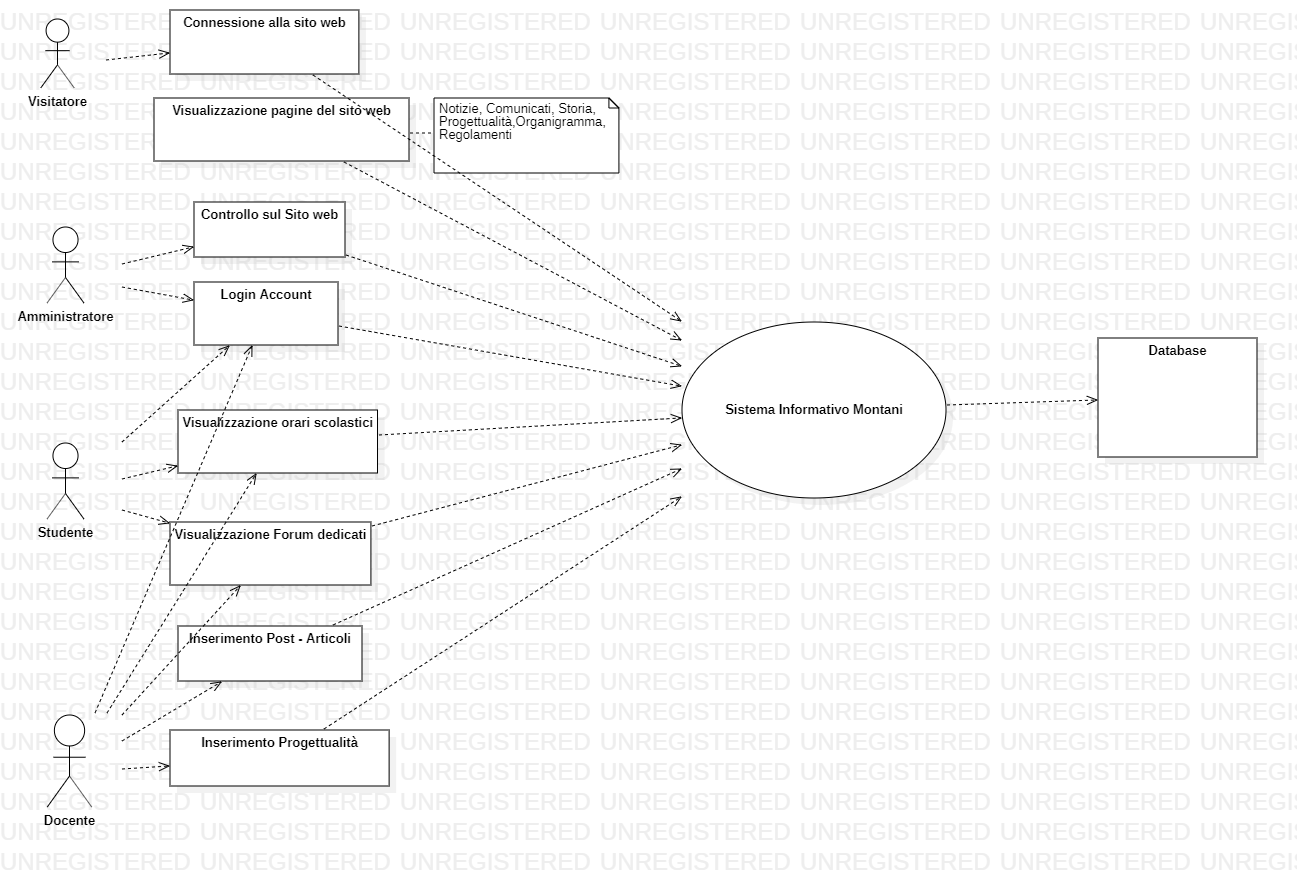
\includegraphics[scale=0.35]{UseCaseDiagram.png}
	Per l'implementazione di una sezione dedicata alle progettualità è stata definito un'entità progetto. Un progetto si compone di un identificativo progetto, un nome progetto, un obiettivo, una tipologia progetto (PCTO, Scuola e Territorio,...), una descrizione progetto ed eventuali link allegati. I progetti possono essere visualizzati da qualsiasi tipologia di utente. I progetti possono essere caricati da utenti con permessi Docente. Un progetto sarà inoltre associato a una classe dell'Istituto. Una classe dell'Istituto sarà identificata da un'identificativo, una denominazione e un anno scolastico. Un anno scolastico identificherà univocamente la classe nel tempo.

	\subsection{\textbf{Browser supportati}}

	\subsection{\textbf{Ottimizzazioni al motore di ricerca}}
	SEO, ....	
\clearpage
	
\section{\textbf{Ulteriori specifiche}}
Ulteriori specifiche, se necessarie, verranno aggiunte nelle prossime versioni del seguente documento.
\end{document}
	
    